\documentclass[]{IEEEtran}

\title{Modellazione in SystemC di un sistema hardware/software per il controllo del livello dell'acqua in un serbatoio}
\author{Vladislav Bragoi - VR436747}

\usepackage{graphicx}
\usepackage[utf8]{inputenc}
\usepackage[italian]{babel}
\usepackage{booktabs}
\usepackage{float}
\usepackage{caption}
\usepackage{tikz}
\usetikzlibrary{shapes,arrows}
\newcommand{\state}[1]{\textit{#1}}
\newcommand{\code}[1]{\texttt{#1}}
\renewcommand{\arraystretch}{1.2}
 % \setlength{\tabcolsep}{0.5em}
\begin{document}
\maketitle

\begin{abstract}
Questo documento presenta l'implementazione ai fini didattici, di un sistema per il controllo del livello dell'acqua in 
un serbatoio, con sviluppo di moduli SystemC a vari livelli di descrizione hardware/software.
\end{abstract}

\section{Introduzione} \label{sec:intro}
\begin{figure}[bt]
	\centering
	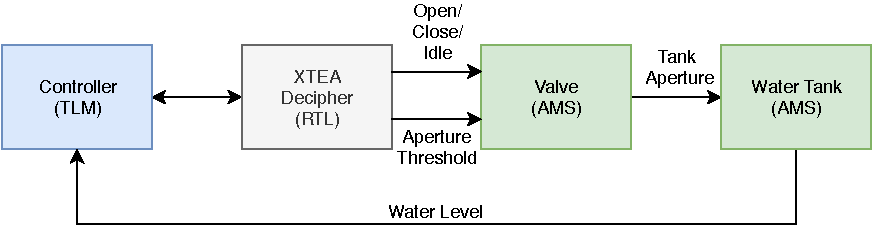
\includegraphics[width=\columnwidth]{figures/system.pdf}
	\caption{Organizzazione in moduli del sistema.}
	\label{fig:system}
\end{figure}

Il sistema descritto in questo documento deve monitorare e controllare il livello dell'acqua in un serbatoio. La figura 
\ref{fig:system} ne mostra la struttura, organizzata nei seguenti moduli:
\begin{itemize}
    \item Controller, si occupa di leggere il livello dell'acqua ricevuto dal serbatoio (Water Tank), e di inviare sulla 
    base di questo livello un comando al modulo Valve, attraverso l'XTEA Decipher, in modo da attuare il controllo 
    sull'apertura della valvola, regolando di conseguenza il livello dell'acqua nel serbatoio. Da notare che questo 
    modulo cifra tutte le informazioni prima di inviarle agli altri moduli.
    
    \item XTEA Decipher, si occupa di decifrare i messaggi ricevuti dal Controller secondo l'agoritmo eXtended TEA 
    (interessante in questo caso poich\'e utilizza poche risorse hw, adattandosi perfettamente a questo tipo di sistema 
    embedded), per poi inviarli direttamente al modulo che svolge la funzione di attuatore, regolando i gradi di apertura
    della valvola.
    
    \item Valve, applica i comandi che gli vengono inviati dal Controller attraverso l'Xtea Decipher, e modifica 
    l'apertura/chiusura della valvola per far riempire il serbatoio.
    
    \item Water Tank, \`e il sistema dinamico che si occupa del controllo dell'acqua sulla base della seguente funzione:
     \[\dot{x} = 0.6 * a - 0.03 * x\]
     dove $a$ \`e l'apertura della valvola e $x$ \`e il livello dell'acqua.
\end{itemize}

Il sistema da progettare segue diverse implementazioni prima del suo completamento nella versione finale chiamata 
"Heterogeneous Platform". In particolare, occorre sviluppare i vari sottomoduli seguendo diversi stili di progettazione,
con un'implementazione dei singoli a diversi livelli di astrazione.

Nella subdirectory HW\_Subsystem vengono raccolte le diverse implementazioni del modulo XTEA, che hanno permesso di estrarre
le principali caratteristiche della progettazione digitale e che vengono presentate nella sezione~\ref{sec:xtea}, mentre 
nella subdirectory Continous\_Subsystem viene presentata un'implementazione delle componenti analogiche (a tempo continuo 
e a tempo discreto) del sistema, e che verranno descritte nella sezione~\ref{sec:continuous}.

Come sar\`a possibile verificare in seguito, l'implementazione modulare dei vari componenti ne permette sia una 
progettazione in SystemC (linguaggio di descrizione hw/sw di riferimento per questo progetto), sia la possibilit\`a di 
simulare tutti i componenti eterogenei nel loro insieme.

\section{Background}
Il sistema \`e stato implementato interamente in C++, utilizzando la libreria SystemC, poich\'e una delle motivazioni 
principali all'utilizzo di questa libreria \`e quello di poter integrare e simulare i vari componenti assieme, sviluppati 
a diversi livelli di astrazione. In particolare, i livelli di astrazione utilizzati sono:
\begin{itemize}
    \item SystemC RTL\cite{RTL} (Register Transfer Level), per una modellazione a basso livello, e dunque pi\`u vicina 
    all'hardware, con sviluppo dei moduli suddividendo la parte di logica di controllo, (\textit{fsm}), dalla parte che 
    esegue i calcoli e le operazioni aritmetiche/logiche (\textit{datapath}).
    
    \item SystemC\cite{SystemC} TLM (Transaction-level Modeling), che permette di descrivere come i vari moduli 
    interagiscono tra loro, grazie ai diversi stili messi a disposizione dalla libreria, ovvero TLM AT 
    (approximately-timed) e TLM LT (loosely-timed) per una sincronizzazione basata su chiamate non bloccanti e/o basata 
    sul concetto del temporal decoupling rispettivamente ai due stili, per arrivare ad una sincronizzazione a chiamate 
    bloccanti in cui non si tiene traccia del tempo di simulazione, e dunque molto pi\`u vicina ad una descrizione 
    algoritmica, coincidente con lo stile TLM UT (untimed).
    
    \item SystemC AMS\cite{AMS} (Analog/Mixed-Signal), che permette di modellare componenti analogiche e/o mixed-signal 
    utilizzando diversi tipi di formalismi quali TDF (Timed Data Flow) per una modellazione non conservativa di sistemi 
    a tempo discreto, LSF (Linear Signal FLow) per una modellazione non conservativa di sistemi a tempo discreto e a 
    tempo continuo (utilizzando solver automatici per risolvere le equazioni differenziali o alle differenze che 
    descrivono il sistema), e ELN (Electrical Linear Network) per una modellazione conservativa di sistemi a tempo 
    continuo.
\end{itemize}

\section{Metodologia applicata}

Le specifiche del progetto richiedevano di strutturare il sistema in moduli che possano essere implementati secondo i 
diversi livelli di astrazione messi a disposizione dalla libreria SystemC. Di seguito verranno illustrate nel dettaglio 
le caratteristiche di ciascun modulo:

\subsection{Xtea [RTL/TLM]}\label{sec:xtea}
Il modulo XTEA implementa l'agoritmo eXtended TEA, ideato da David Wheeler e Roger Needham al Cambridge Computer 
Laboratory. Il vantaggio principale di questo algoritmo \`e quello di avere una struttura semplice per poter essere 
impiegato in sistemi di limitate risorse hardware, e quindi il suo impiego si adatta perfettamente ad un sistema embedded
semplice quale quello che stiamo modellando, per poter offrire un minimo livello di sicurezza. A partire dai sorgenti i
n C/C++ \`e stato possibile ricavare la seguente struttura di base: 
\begin{figure}[h]
    \centering
    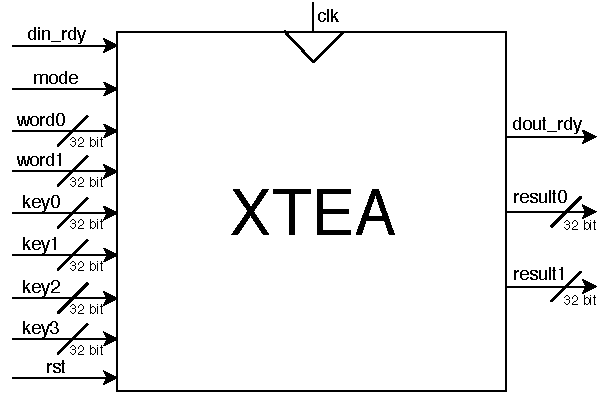
\includegraphics[width=0.7\columnwidth]{figures/xtea.pdf}
	\caption{Struttura generale del modulo XTEA}
    \label{fig:xtea}
\end{figure}

Di seguito vengono descritti i diversi livelli di astrazione in cui il modulo \`e stato implementato:
\begin{itemize}
    \item XTEA RTL, descritto in SystemC RTL, \`e stato progettato suddividendo (in base a quanto detto precedentemente) 
    la parte di controllo dalla parte relativa ai calcoli. In figura~\ref{fig:fsmd} vengono presentate le porte di 
    ingresso e di uscita del modulo e i segnali che interconnettono l'FSM al Datapath. In particolare, l'FSM è sensibile
    alle variazioni sul segnale \state{din\_rdy} e \state{status}, mentre utilizza \state{mode} e \state{counter} per 
    decidere lo stato prossimo. Il Datapath invece è sensibile ai segnali di \state{reset} e \state{clock}, e utilizza 
    \state{mode}, \state{word\_0}, \state{word\_1} per calcolare i valori di output \state{result\_0} e \state{result\_1}. 
    Per quanto riguarda i segnali interni, nel datapath vengono definiti i seguenti:
    \begin{itemize}
        \item \state{k}, segnale a 2 bit per memorizzare quale delle 4 chiavi in input utilizzare nel calcolo;
        \item \state{key}, segnale a 32 bit per memorizzare temporaneamente la chiave da utilizzare;
        \item \state{delta}, per memorizzare il valore del parametro delta;
        \item \state{sum}, segnale a 64 bit utilizzato per i calcoli ad ogni iterazione;
        \item \state{counter}, segnale a 7 bit, utilizzato per le 64 iterazioni del ciclo per le due modalità (il motivo 
        per cui è stato scelto di effettuare 64 iterazioni invece di 32 verrà chiarito più avanti). Sono sufficienti 6 
        bit per compiere 64 iterazioni ma poiché all'ultima iterazione il segnale viene ulteriormente incrementato di 
        una unità, questo dev'essere a 7 bit per non perdere di informazione;
        \item \state{v0} e \state{v1}, segnali di appoggio per i calcoli, a 32 bit.
    \end{itemize}
    Nella descrizione del modulo secondo la EFSM\footnote{Extended Finite State Machine} in figura \ref{fig:efsm} (in 
    appendice), la parte di logica di controllo \`e rappresentata dalle transizioni e dalle condizioni sulle transizioni, 
    mentre il Datapath \`e rappresentato dagli stati dell'automa. A partire dagli stati \state{ST\_M0}, \state{ST\_K}, 
    \state{ST\_CALC} e \state{ST\_SUM} per la modalit\`a di cifratura (e equivalentemente \state{ST\_M1}, \state{ST\_K}, 
    \state{ST\_CALC} e \state{ST\_SUM} per la modalit\`a di decifratura) \`e possibile vedere come sia stato scelto, a 
    differenza della versione dell'algoritmo di C/C++, di effettuare un numero pari a 64 iterazioni per poter 
    riutilizzare i blocchi che altrimenti sarebbero ripetuti per le due modalit\`a. Inoltre, per quanto riguarda lo stato 
    \state{ST\_CALC} che tra tutti sembrerebbe essere quello a complessit\`a pi\`u alta, \`e stato scelto di non 
    spezzarlo in due stati in quanto le operazioni al suo interno risutano essere molto simili, e dunque un'eventuale 
    ottimizzazione dell'area secondo gli algoritmi allo stato dell'arte ne ridurrebbe drasticamente sia la complessit\`a, 
    sia gli elementi hardware da impiegare.
    
    \begin{figure}[bt]
        \centering
        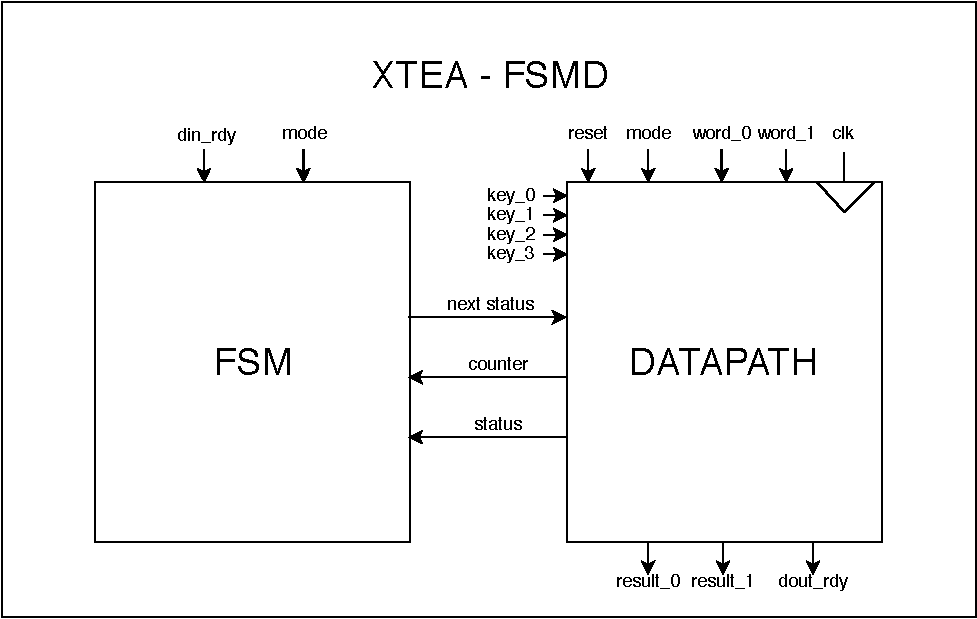
\includegraphics[width=0.9\columnwidth]{figures/fsmd.pdf}
        \caption{FSMD del modulo XTEA RTL}
        \label{fig:fsmd}
    \end{figure}

    \item XTEA TLM \`e la versione di XTEA sviluppata in SystemC TLM (nelle relative varianti UT, LT e AT4). La 
    struttura cha accomuna tutti e tre i moduli è la seguente: il \emph{testbench} (che implementa l'interfaccia 
    \code{tlm\_bw\_transport\_if}) effettua la funzionalit\`a dell'initiator, ovvero esegue le chiamate alla controparte 
    \emph{xtea} (che di conseguenza effettua la funzionalit\`a del target, implementando l'interfaccia 
    \code{tlm\_fw\_transport\_if}), avviando transazioni per permettere lo scambio di messaggi, che in questo caso, 
    corrispondono all'invio dei dati da cifrare/decifrare. In particolare, ad ogni transazione viene inviato un payload 
    esteso, ovvero un payload con allegate le informazioni definite nella struttura \code{iostruct}, che racchiude gli 
    input e gli output definiti nella struttura generica del modulo in figura~\ref{fig:xtea}. 
    
    Di seguito vengono presentate le diverse versioni, dalla pi\`u specifica alla pi\`u astratta:
    \begin{itemize}
        \item TLM Aproximately Timed (4 phases), è la versione basata su chiamate non bloccanti. La sincronizzazione 
        avviane secondo il classico protocollo di handshake a 4 fasi, in particolare il \emph{testbench} invia i dati 
        alla parte \emph{xtea} mettendosi successivamente in attesa dell'acknowledgement (fasi \code{BEGIN\_REQ}, 
        \code{END\_REQ}), \emph{xtea} riceve la transazione, elabora i dati e ne salva il risultato, per poi successivamente 
        ritornare l'acknowledgement alla controparte sbloccandone l'esecuzione (fasi \code{BEGIN\_RESP}, 
        \code{END\_RESP}).
        \item Loosely Timed, \`e la versione basata su una sincronizzazione a chiamate bloccanti. Qui l'initiator (che, 
        come detto sopra, è il \emph{testbench}) chiama la funzione \code{b\_transport} implementata nel target, 
        aggiungendo alla transazione, oltre al payload per lo scambio dei messaggi, anche l'informazione relativa al 
        tempo. Questa viene utilizzata per sfruttare il cosidetto Temporal Decoupling, ovvero per permettere ai processi 
        (nel nostro caso il testbench) di continuare la propria esecuzione senza per\`o incrementare il tempo di 
        simulazione, per poi sincronizzarsi esplicitamente in punti definiti oppure allo scadere del quanto di tempo 
        che gli è stato associato dallo scheduler, riducendone cos\`i il tempo totale della simulazione.
        \item TLM Untimed \`e una versione simile alla precedente, in cui non viene per\`o specificata l'informazione 
        relativa al tempo. Non richiede dunque una sincronizzazione esplicita, poich\`e questa viene garantita dalla 
        chiamata bloccante alla \code{b\_transport}, permettendo una classica sincronizzazione dei processi.
    \end{itemize}
\end{itemize}
La differenza tra queste quattro versioni sta nel tempo di simulazione. In tabella \ref{tab:time} vengono presentate le 
statistiche di simulazione basate su un'esecuzione di 1000 iterazioni per modulo, le quali mettono in evidenza come la 
versione RTL richieda più tempo di simulazione rispetto alle altre, poich\`e \`e la versione di XTEA pi\`u precisa, 
ovvero quella che garantisce una sincronizzazione tra le parti pi\`u accurata. Gli altri moduli (TLM), essendo meno 
accurati in termini di sincronizzazione, impiegano meno tempo di simulazione, con una differenza che cala gradualmente 
con l'aumento del livello di astrazione.
\begin{table}[]
    \centering
    \begin{tabular}{lllll}
    \toprule
                & UT     & LT     & AT4    & RTL    \\ \hline
    Real time   & 0,039s & 0,045s & 0,069s & 1,025s \\
    User time   & 0,009s & 0,015s & 0,016s & 0,894s \\
    System time & 0,018s & 0,018s & 0,044s & 0,052s \\ \bottomrule
    \\
    \end{tabular}
    \caption{Statistiche di esecuzione di XTEA secondo i diversi livelli di astrazione}
    \label{tab:time}
\end{table}

\subsection{Wwatertank System [AMS]}\label{sec:continuous}

Water Tank System è un sistema per il controllo e il monitoraggio del livello dell'acqua di un serbatoio. La modellazione,
che segue la struttura presentata in figura \ref{fig:continuous_system}, ha richiesto l'utilizzo di SystemC AMS, poich\'e 
i componenti da modellare presentano tutti comportamenti a tempo discreto e/o a tempo continuo.
\begin{figure}[bt]
	\centering
	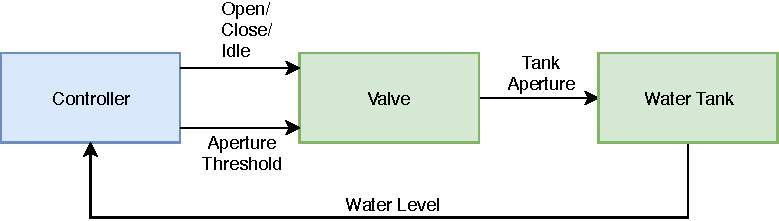
\includegraphics[width=\columnwidth]{figures/countinous_system.pdf}
	\caption{Struttura del watertank system}
	\label{fig:continuous_system}
\end{figure}
In particolare, il Controller, descritto in SystemC AMS utilizzando il formalismo TDF per una modellazione a tempo discreto, 
deve leggere il livello dell'acqua fornitogli in input e deve poi verificare che stia dentro il range $[5 \dots 8.8]$. 
Inoltre, sulla base delle condizioni riportate in tabella \ref{tab:behaviour}, il modulo deve periodicamente inviare al 
suo immediato vicino un comando di apertura o chiusura della valvola per fare riempire il serbatoio, e una threshold per 
indicare il livello di apertura massima che la valvola deve raggiungere. Dell'attuazione del comando si occuper\`a il 
modulo Valve, descritto anche questo secondo il formalismo TDF non conservativo per una modellazione a tempo discreto, 
mentre il modulo Water Tank è il componente che rileva il livello dell'acqua. Il suo comportamento rispecchia il seguente 
modello matematico, rappresentato sotto forma di schema a blocchi, e dunque si è scelto di descriverlo utilizzando 
il formalismo LSF non conservativo a tempo continuo, che aiuta nella risoluzione dell'equazione differenziale associata 
al modello grazie ai solver automatici che la libreria mette a disposizione:\\

\begin{table}[]
    \centering
    \begin{tabular}{lll}
    \toprule
    Water level     & Command   & Aperture threshold\\ \hline
    $range(5,8.8)$  & IDLE      & - \\
    $>8.8$          & CLOSE     & $t = t * 0.7$\\
    $<5$            & OPEN      & $t = t * 1.1$\\ \bottomrule
    \\
    \end{tabular}
    \caption{Parametri che influenzano il controllo sulla valvola}
    \label{tab:behaviour}
\end{table}  

\tikzstyle{block} = [draw, rectangle, minimum height=3em, minimum width=5em]
\tikzstyle{sum} = [draw, circle, node distance=1cm]
\tikzstyle{input} = [coordinate]
\tikzstyle{output} = [coordinate]

\resizebox{0.95\columnwidth}{!}{%
\begin{tikzpicture}[auto, node distance=1.5cm,>=latex']
    \node [input, name=input] {};
    \node [block, right of=input] (k1) {0.6};
    \node [sum, right of=k1, node distance=2.3cm] (sum) {};
    \node [block, right of=sum, node distance=1.8cm] (integral) {$\int$};
    \coordinate [right of=integral] (tmp);
    \node [block, below of=integral, node distance=1.5cm] (k2) {0.03};
    \node [output, right of=tmp] (output) {};
    \coordinate [below of=tmp] (tmp1);
    \coordinate [below of=sum] (tmp2);

    \draw [draw,->] (input) -- node {$a$} (k1);
    \draw [->] (k1) -- node {$sig_1$} (sum);
    \draw [->] (sum) -- node {$x'$} (integral);
    \draw [->] (integral) -- node {} (tmp) -- node [name=y] {$x$}(output);;
    \draw [->] (tmp) |- (tmp1) |- node {} (k2);
    \draw [->] (k2) -| (tmp2) -| node {$sig_2$} (sum);
\end{tikzpicture}
}
Ai capi di questo modello sono stati posizionati (in input e in output) dei convertitori da TDF a LSF e da LSF a TDF per
potersi interfacciare con gli altri moduli (descritti in SystemC AMS-TDF appunto) a tempo discreto.
Inoltre, per evitare problemi dovuti al loop creato, \`e stato inserito un delay sulla porta water\_level del Controller.

Per quanto riguarda la stabilizzazione dell'acqua, questa, come mostrato in figura \ref{fig:water_continuous_system}, 
si stabilizza approsimativamente attorno ai 200 secondi.
\begin{figure}[t]
	\centering
	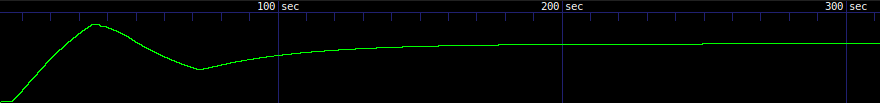
\includegraphics[width=0.95\columnwidth]{figures/water_level_continuous_subsystem.png}
	\caption{Stabilizzazione dell'acqua relativamente al Water Tank System (AMS) - Continous Subsystem}
	\label{fig:water_continuous_system}
\end{figure}

\subsection{Heterogeneous Platform}

\begin{figure*}[b]
    \centering
    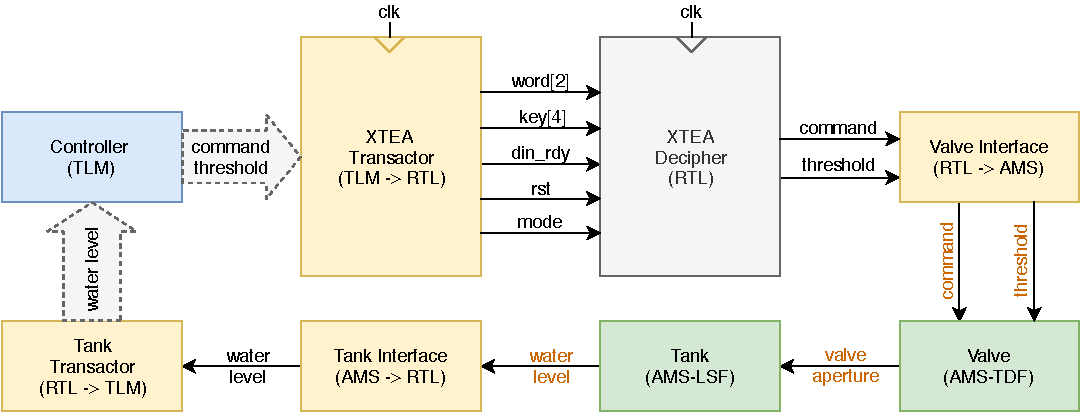
\includegraphics[width=0.8\textwidth]{figures/heterogeneous.pdf}
    \caption{Struttura del heterogeneous platform}
    \label{fig:heterogeneous}
\end{figure*}

L'Heterogeneous platform, ovvero l'unione in un unico sistema di tutti i moduli visti fin'ora (descritti ognuno secondo 
un proprio livello di astrazione) e gi\`a presentato in parte nella sezione \ref{sec:intro}, \`e costituito da ulteriori 
4 componenti, necessari per poterne simulare tutto l'insieme: i transattori. 
In figura \ref{fig:heterogeneous} \`e possibile vedere come questi nuovi componenti trasformano un segnale di 
interconnessione tra i singoli moduli:
\begin{itemize}
    \item da TLM a RTL, per i segnali che partono dal Controller (in TLM) e che vengono 
    inviati al modulo Xtea Decipher (in RTL);
    \item da RTL a AMS, per i segnali che partono dal modulo Xtea Decipher e che entrano nel 
    modulo Valve (in AMS);
    \item da AMS a RTL e nuovamente a TLM, per i segnali in uscita dal modulo Tank (in AMS) ed entranti nel modulo 
    Controller (descritto in TLM);
\end{itemize}
Da notare che i segnali di colore nero in figura sono segnali RTL, mentre quelli di colore arancio sono segnali AMS. 
Invece i segnali rappresentati dalle frecce tratteggiate rappresentano transazioni TLM.
Inoltre, i componenti Valve Interface e Tank Interface sono interfacce RTL necessarie per poter 
far comunicare tra loro moduli scritti in TLM, con moduli scritti in AMS e viceversa, mentre il modulo Valve Interface 
contiene al suo interno una parte di logica per riconoscere quando l'Xtea Decipher gli invia un comando oppure una 
threshold. Queste informazioni infatti, sono inviate in due momenti separati e servono per poter utilizzare lo stesso 
componente in modo da decifrare due tipologie di informazione diverse che gli vengono passate.
Infine, il Controller essendo descritto in SystemC TLM, \`e l'initiator sia del modulo Tank Transactor, sia del modulo 
Xtea Transactor (che sono a loro volta di tipo target), poich\`e tale configurazione permette di gestire meglio la 
sincronizzazione del loop di controllo direttamente nel modulo Controller.


\section{Risultati}

\begin{figure*}[tb!]
	\centering
	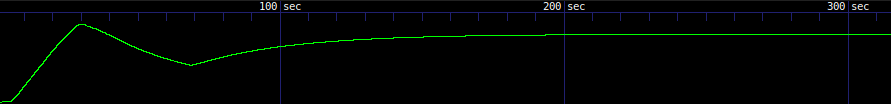
\includegraphics[width=0.8\textwidth]{figures/water_level_heterogeneous.png}
	\caption{Stabilizzazione dell'acqua del sistema eterogeneo}
	\label{fig:water_heterogeneous}
\end{figure*}
\begin{figure*}[tb!]
	\centering
	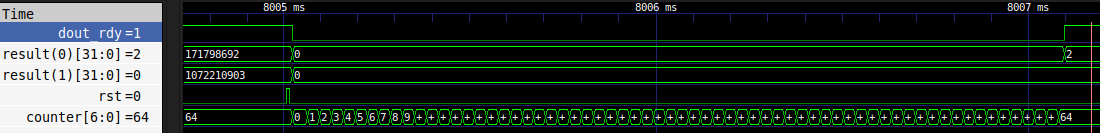
\includegraphics[width=0.8\textwidth]{figures/rtl_signals.png}
	\caption{Valori dei segnali nel modulo XTEA RTL}
	\label{fig:rtl_sig}
\end{figure*}

La corretta funzionalit\`a del sistema \`e stata testata a partire dai singoli moduli. Questi infatti sono stati 
sottoposti a diversi testbench per verificarne il comportamento individuale prima di poter essere integrato con gli altri
moduli. Inoltre, in alcuni casi \`e stato necessario utilizzare anche il debugger, come ad esempio per la versione RTL di 
XTEA che ha permesso di risolvere alcuni dei problemi legati alla sincronizzazione e scrittura sui vari segnali.
Successivamente \`e stata testata la comunicazione tramite transazioni TLM, ad esempio per la comunicazione tra
Controller e Xtea Transactor. 

Infine, il sistema eterogeneo è stato sviluppato seguendone il flusso di esecuzione utilizzando i file di tracing dei 
segnali, che permettono di tracciare l'intero flusso rispettando per\`o i reali tempi di esecuzione dell'intero sistema.
La figura~\ref{fig:rtl_sig} riporta infatti i tempi relativi all'esecuzione di un ciclo di decifratura del modulo XTEA RTL,
che impiega - come ben visibile in figura - poco pi\`u di 2 millisecondi.
Mettendo in relazione questo risultato con quello ottenuto dalla stabilizzazione del livello dell'acqua in 
figura~\ref{fig:water_heterogeneous}, \`e possibile vedere infatti, oltre all'evidente stabilizzazione del livello ad un
valore pari a 8.5 c.a., che l'esecuzione modulo RTL \`e molto pi\`u veloce rispetto agli altri moduli del sistema (questo
perché il modulo lavora alla frequenza del clock essendo il componente descritto a pi\`u basso livello di astrazione,
quindi pi\`u vicino all'hardware).

In riferimento ai tempi di simulazione invece, poich\'e per una co-simulazione di diversi modelli descritti a diversi 
livelli di astrazione \`e richiesta una maggiore complessit\`a di sincronizzazione, l'esecuzione totale dell'intero 
sistema risulta essere piuttosto lenta. Questo perch\'e occorre sincronizzare i moduli TLM che sono meno accurati e che 
permettono per\`o una simulazione pi\`u veloce, con il modulo XTEA RTL, che, come gi\`a visto in tabella \ref{tab:time} 
richiede pi\`u tempo di simulazione dovuto alla sua maggior precisione (poich\'e viene simulato il comportamento del modulo ad
ogni ciclo di clock).


\section{Conclusioni}
Il riuso dei vari componenti per ridurre il cosidetto TTM (Time to Market) permette di costruire in breve tempo un 
prototipo da simulare per poter studiare la fattibilit\`a del progetto nel suo complesso. In particolare, grazie 
all'utilizzo di SystemC \`e stato possibile modellare sia componenti analogiche (a tempo continuo e a tempo discreto), sia 
componenti digitali ed eseguirne una simulazione dell'intero sistema. Questo vantaggio  si \`e mostrato rilevante 
considerando un'eventuale progettazione classica del sistema, in cui si sarebbe dovuto suddividere la parte di 
progettazione hw da quella sw (che ovviamente non sarebbe stata altrettanto fattibile).


\bibliographystyle{IEEEtran}
\bibliography{biblio}

\begin{figure*}[bt]
	\centering
	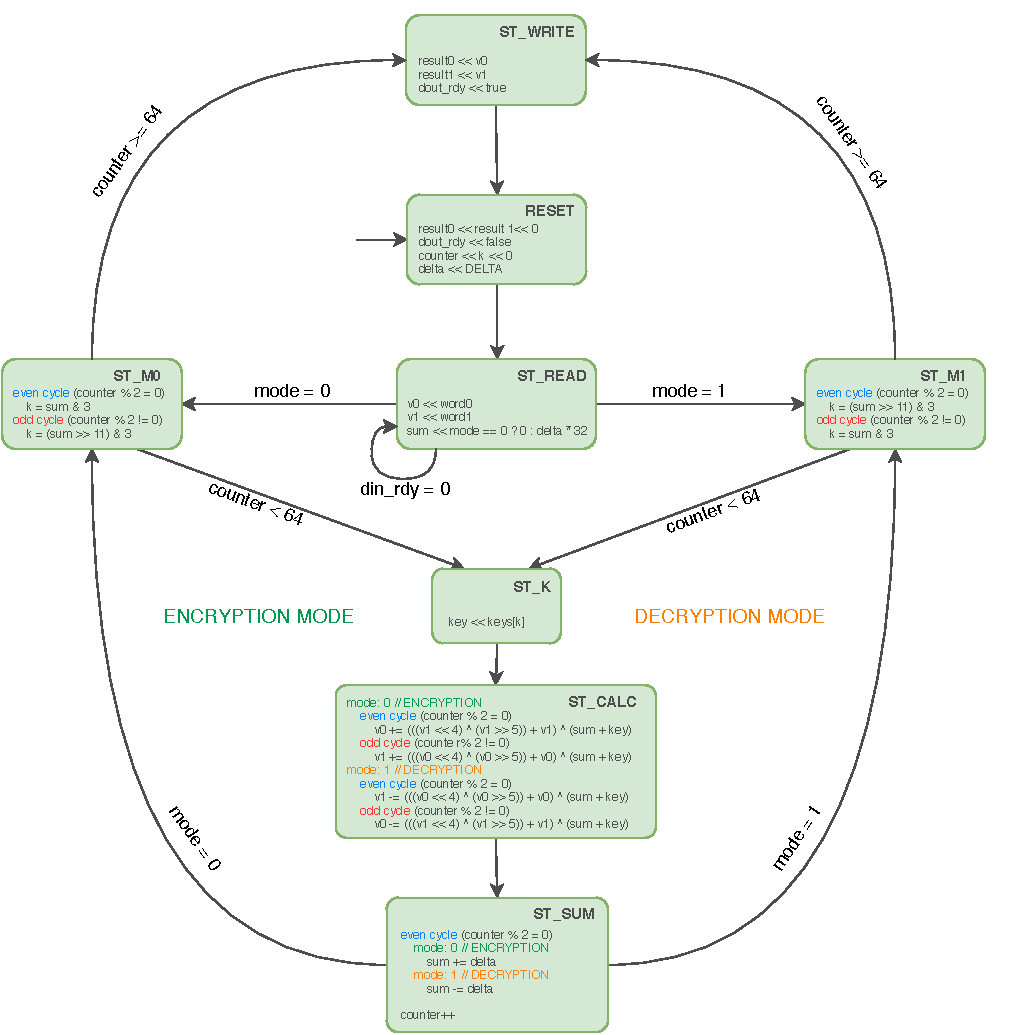
\includegraphics[width=0.7\textwidth]{figures/efsm.pdf}
	\caption{EFSM del modulo XTEA RTL}
	\label{fig:efsm}
\end{figure*}

\end{document}